%%%%%%%%%%%%%%%%%%%%%%%%%%%%%%%%%%%%%%%%%%%%%%%%%%%%%%%%%%%%%%%%%%%%%%%%%%%%%%%%%%%%%%%%%%%%
%%
%% Chapter 1 : Introduction
%%
%%      * Should give an intro/overview of the problem and the context in which it arises
%%      * Then, it should emphasize the problem (problem statement)
%%      * Then the objectives of the proposed research topic and problem
%%      * And finally the organization/structure of the document
%%
%%%%%%%%%%%%%%%%%%%%%%%%%%%%%%%%%%%%%%%%%%%%%%%%%%%%%%%%%%%%%%%%%%%%%%%%%%%%%%%%%%%%%%%%%%%%
\chapter{Introduction}
\label{ch:intro}

%%%%%%%%%%%%%%%%%%%%%%%%%%%%%%%
%   Figures for chapter 1
%%%%%%%%%%%%%%%%%%%%%%%%%%%%%%%

\newcommand{\figDrlLocomotionMotivation}{
    \begin{figure}[!ht]
        \centering
        \begin{subfigure}[b]{0.45\textwidth}
            \centering
            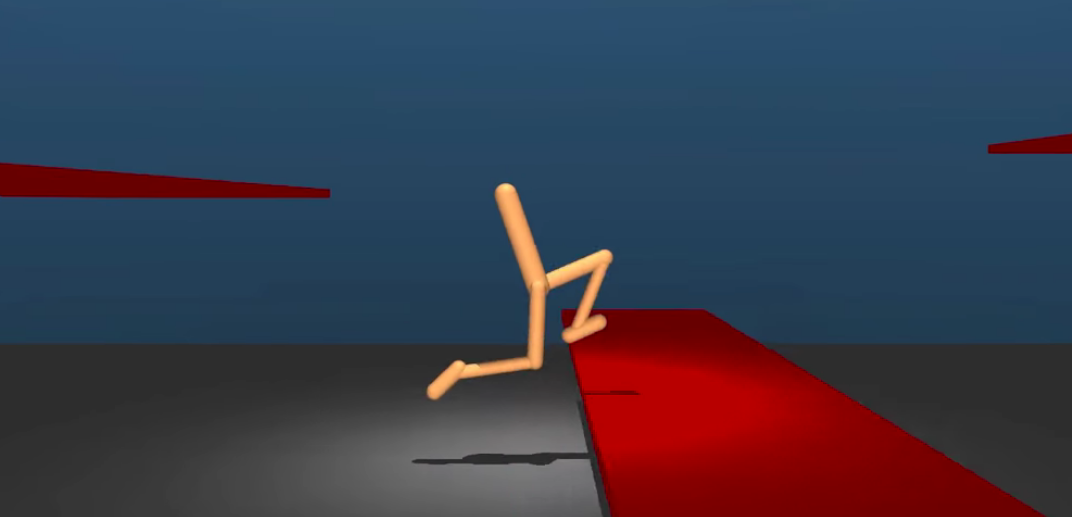
\includegraphics[width=0.9\textwidth]{./chapters/chapter_1/imgs/img_ch1_emergence_of_locomotion.png}
            \caption{}
            \label{fig:ch1_emergence_locomotion}
        \end{subfigure}
        \begin{subfigure}[b]{0.45\textwidth}
            \centering
            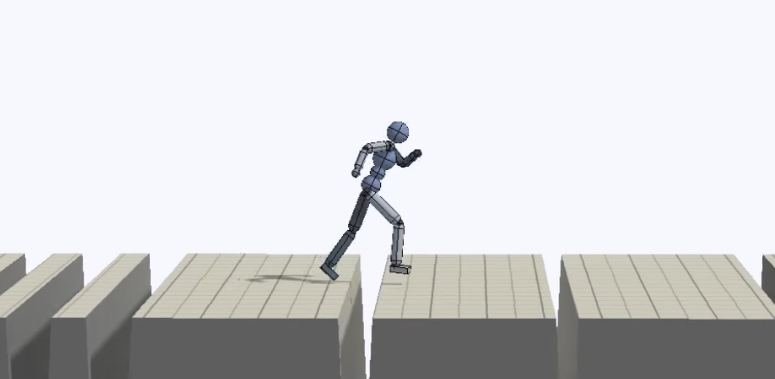
\includegraphics[width=0.9\textwidth]{./chapters/chapter_1/imgs/img_ch1_deepmimic.png}
            \caption{}
            \label{fig:ch1_deepmimic}
        \end{subfigure}
        \caption{Some results from applying Deep Reinforcement Learning to locomotion. 
                    a) Biped traversing simulated environment \citep{DeepmindEmergenceLocomotion}.
                    b) Humanoid traversing simulated environment \citep{DeepMimic} }
        \label{fig:ch1_motivation_drl_locomotion}
    \end{figure}
}

\newcommand{\figDrlBenchmarks}{
    \begin{figure}
        %% Controlsuite
        \centering
        \begin{subfigure}[b]{1.0\textwidth}
            \centering
            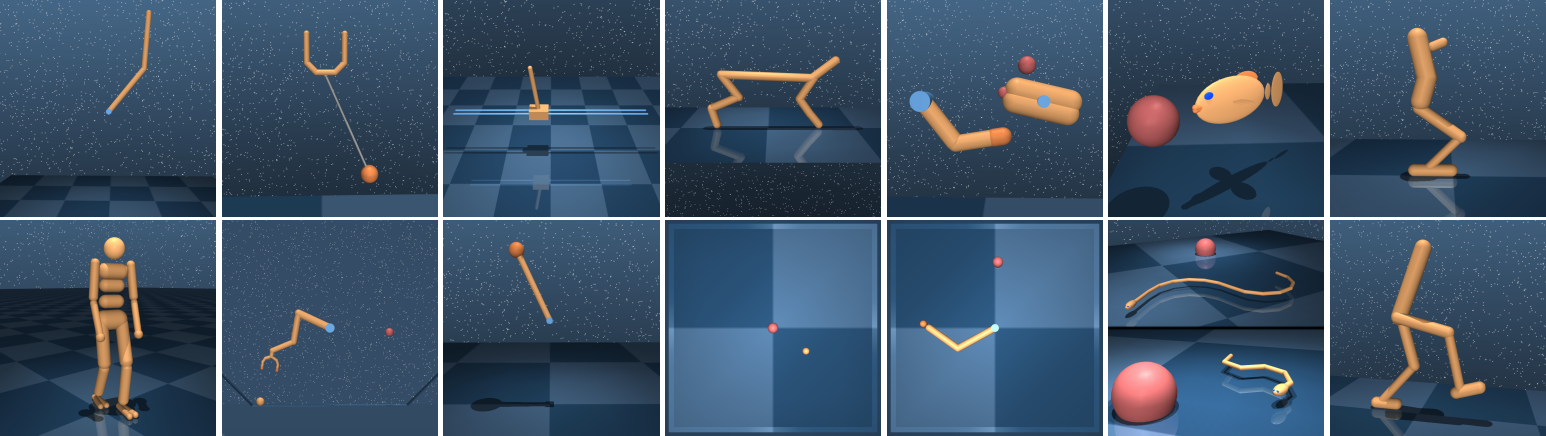
\includegraphics[width=1.0\textwidth]{./chapters/chapter_1/imgs/img_ch1_benchmarks_controlsuite.png}
            \caption{}
            \label{fig:ch1_benchmarks_controlsuite}
        \end{subfigure}
        %% Roboschool
        \centering
        \begin{subfigure}[b]{1.0\textwidth}
            \centering
            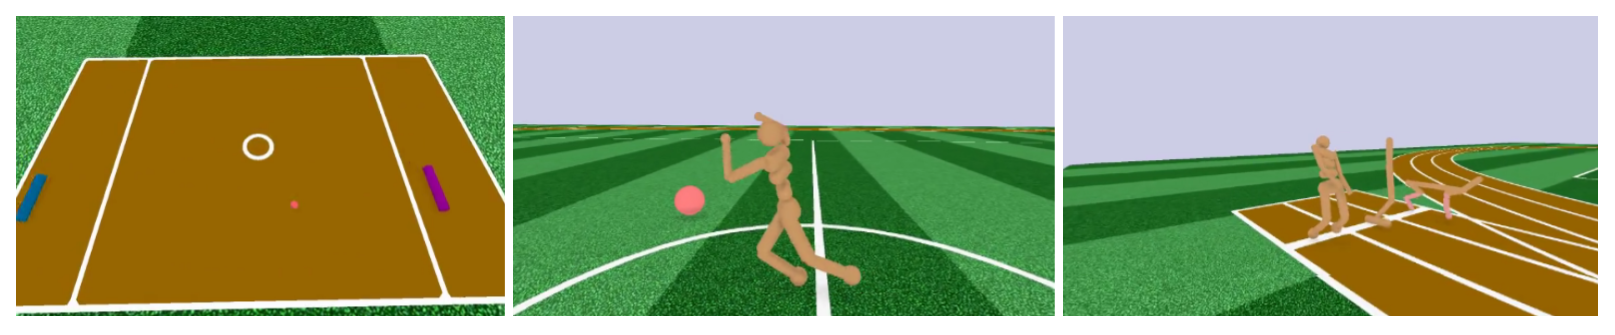
\includegraphics[width=1.0\textwidth]{./chapters/chapter_1/imgs/img_ch1_benchmarks_roboschool.png}
            \caption{}
            \label{fig:ch1_benchmarks_roboschool}
        \end{subfigure}
        %% Gym
        \centering
        \begin{subfigure}[b]{1.0\textwidth}
            \centering
            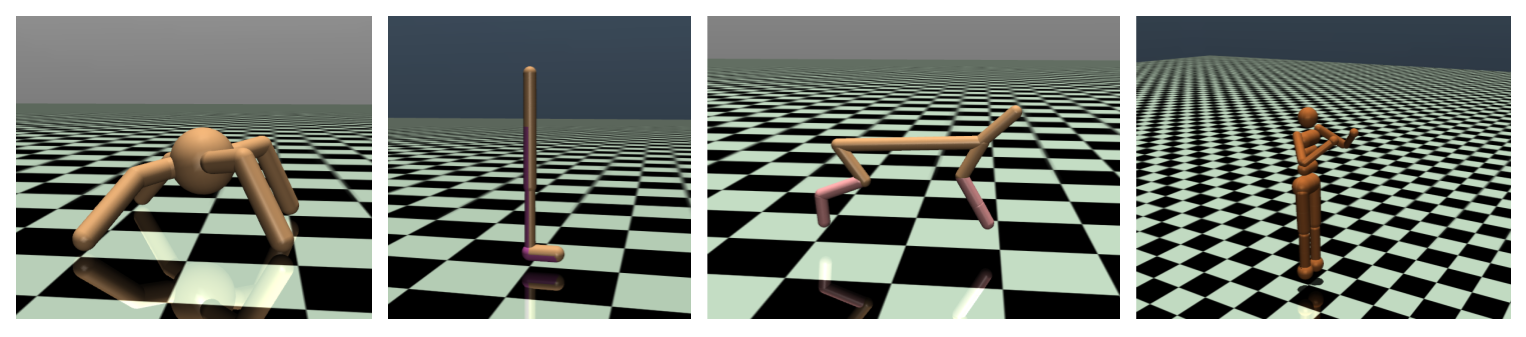
\includegraphics[width=1.0\textwidth]{./chapters/chapter_1/imgs/img_ch1_benchmarks_gym.png}
            \caption{}
            \label{fig:ch1_benchmarks_gym}
        \end{subfigure}
        %% Rllab
        \centering
        \begin{subfigure}[b]{1.0\textwidth}
            \centering
            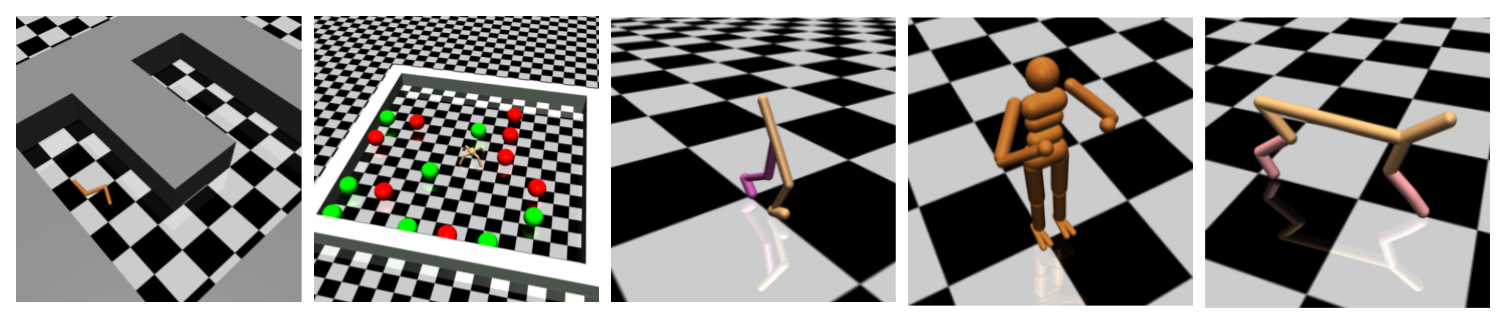
\includegraphics[width=1.0\textwidth]{./chapters/chapter_1/imgs/img_ch1_benchmarks_rllab.png}
            \caption{}
            \label{fig:ch1_benchmarks_rllab}
        \end{subfigure}
        \caption{Available benchmarks for locomotion tasks: 
                            a) controlsuite \citep{Controlsuite},
                            b) roboschool \citep{Roboschool},
                            c) gym \citep{Gym} and
                            d) rllab \citep{Rllab}}
        \label{fig:ch1_drl_locomotion_benchmarks}
    \end{figure}
}

\newcommand{\figEnvironmentsProposalFromTo}{
    \begin{figure}
        \centering
        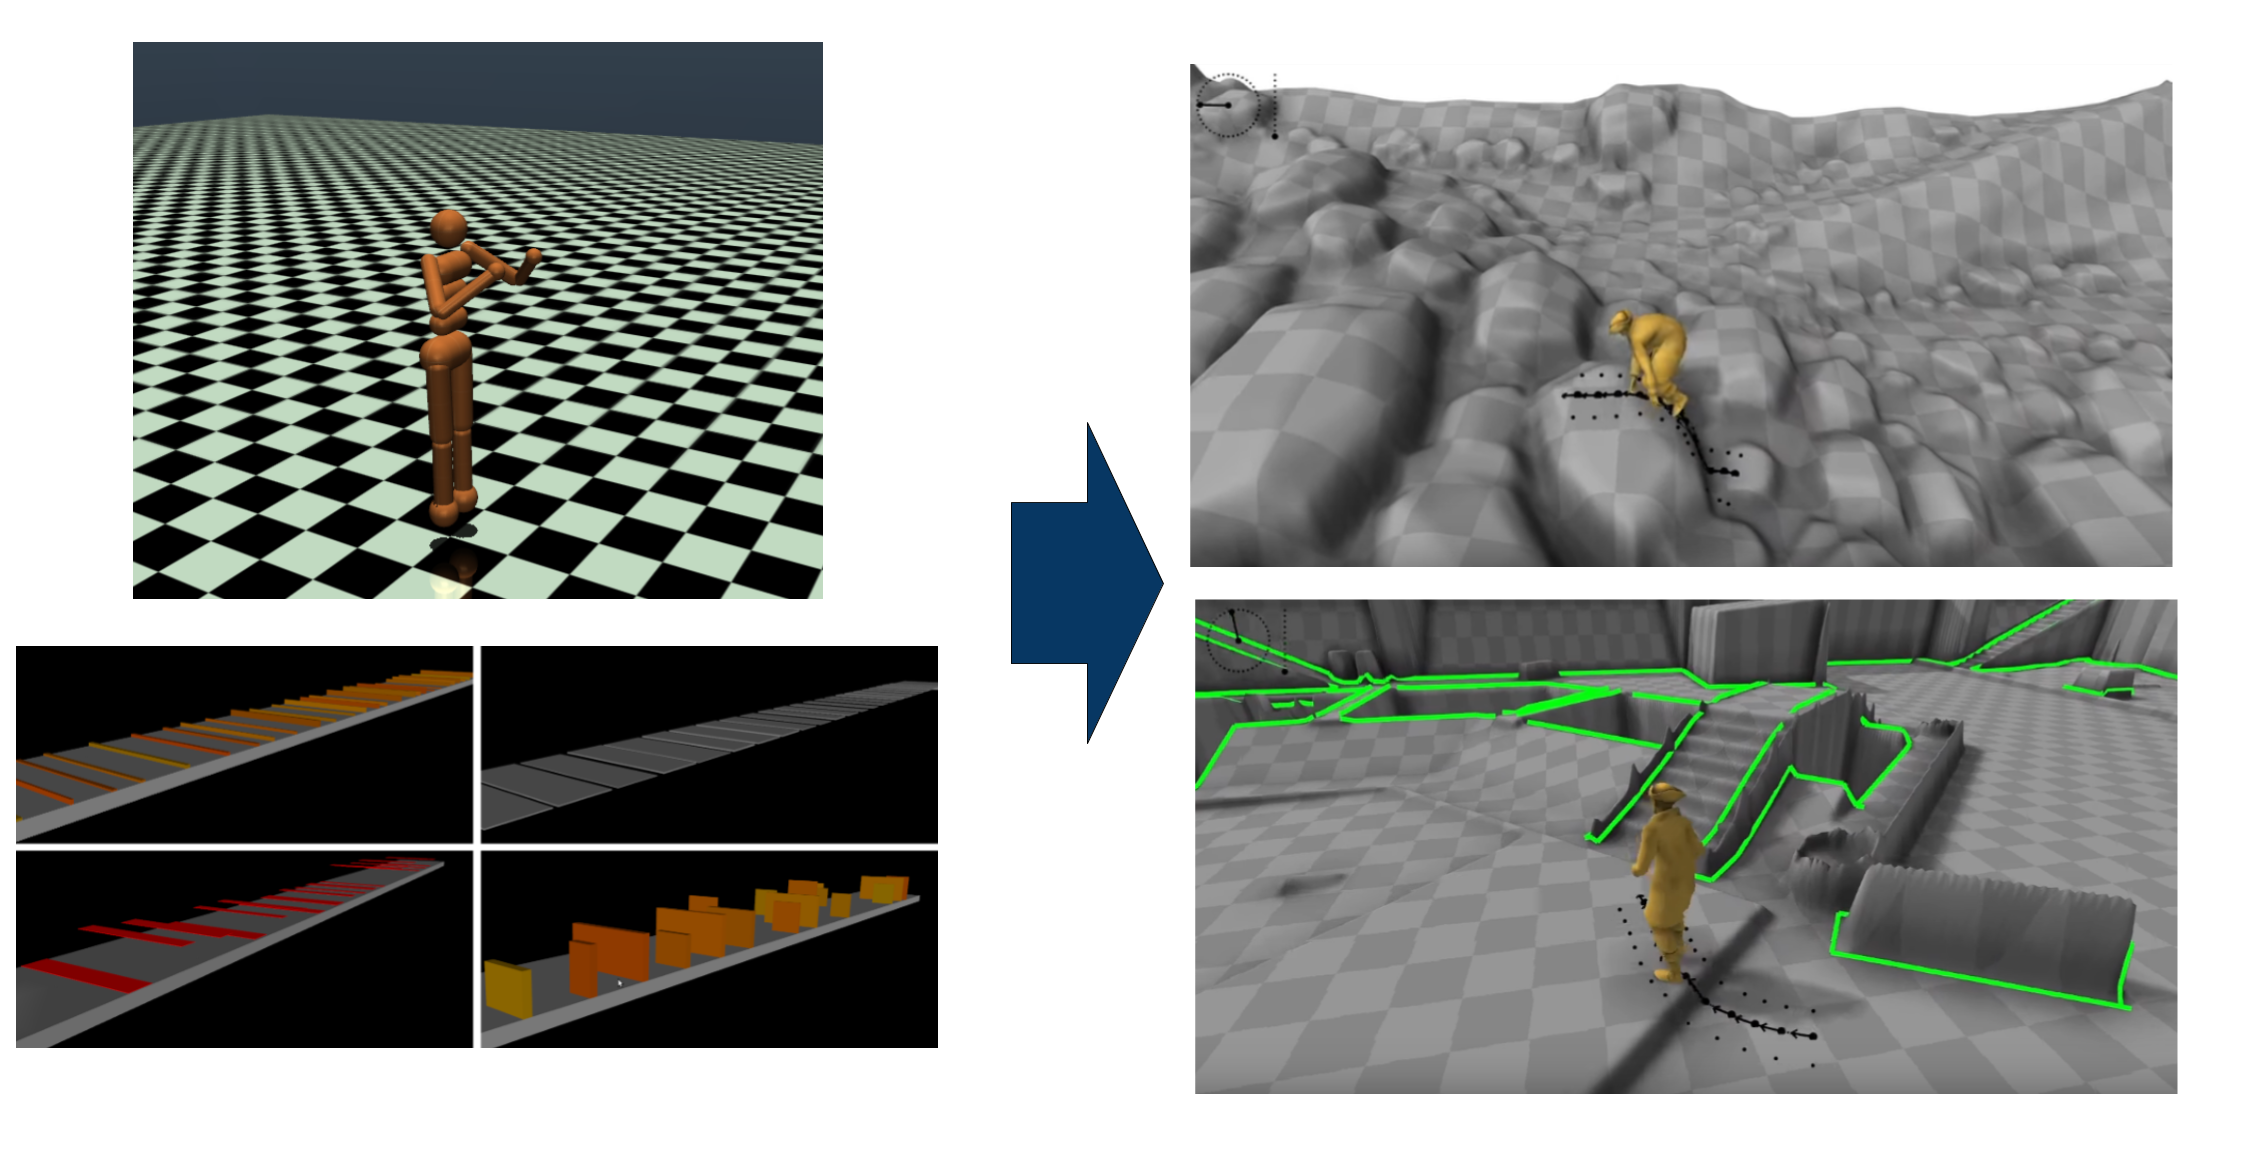
\includegraphics[width=0.8\textwidth]{./chapters/chapter_1/imgs/img_ch1_environments_from_to.png}
        \caption{Comparison of the proposed environments to the environments provided by current benchmarks. 
                 Left: relatively simple environments (image adapted from \citet{Gym}). 
                 Right: relatively more complex proposed environments (images adapted from \citet{Pfnn} ).}
        \label{fig:ch1_environments_comparison_from_to}
    \end{figure}
}

\newcommand{\figEnvManipSimToreal}{
    \begin{figure}
        \centering
        \begin{subfigure}[b]{0.5\textwidth}
            \centering
            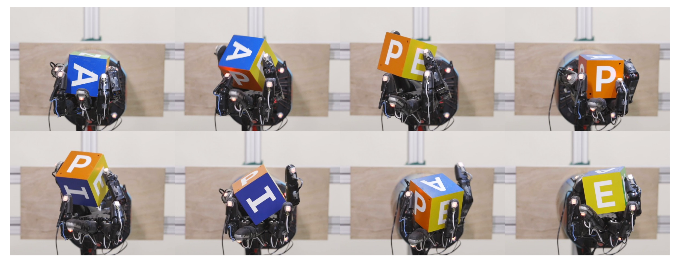
\includegraphics[width=1.0\textwidth]{./chapters/chapter_1/imgs/img_ch1_openai_robot_dexterity.png}
            \caption{}
            \label{fig:ch1_openai_robot_dexterity}
        \end{subfigure}
        \begin{subfigure}[b]{0.5\textwidth}
            \centering
            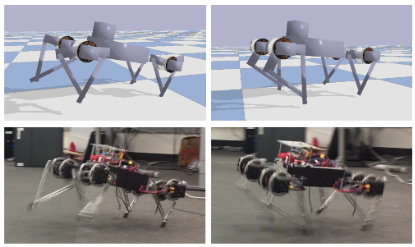
\includegraphics[width=1.0\textwidth]{./chapters/chapter_1/imgs/img_ch1_google_brain_minitaur_sim_to_real.png}
            \caption{}
            \label{fig:ch1_google_brain_minitaur_sim_to_real}
        \end{subfigure}
        \caption{Some examples of sim2real results: 
                            a) Robotic hand generalizing in randomized environment \citep{OpenAISim2real}.
                            b) Quadruped trained in simulation and deployed in real world \citep{GoogleBrainSim2Real} }
        \label{fig:ch1_sim_to_real_approaches}
    \end{figure}
}

Recent advances in the field of Deep Reinforcement Learning (DRL) have achieved good
results in various Reinforcement Learning benchmarks, like the Atari Learning Environment (ALE), 
and the game of Go, just to name a few. These represent discrete action spaces problems, in which 
the action space can be defined by a finite-size set of values. More recently, this approach has also 
been applied to continuous actions spaces, i.e. in continuous control tasks. This has given good results 
in various continuous control benchmarks, like in \citeauthor{DeepmindEmergenceLocomotion}  and \citeauthor{DeepMimic}.

\figDrlLocomotionMotivation

This approach is very promising because it allows the agent to come up with a controller after training in
an environment, which reduces the need to implement highly sophisticated control pipelines. Current available 
environments for training have been presented in various articles (and we will talk more about these in Chapter 2).
Some benchmarks suites are shown in the following figure, and compared to the ones used in the research mentioned previously
they are relatively simpler, consisting mostly of classic control problems and some locomotion tasks in flat terrains.

\figDrlBenchmarks

% @TAG: Refer to content above and "formalize" a bit more
\section{Problem Statement}
\label{sec:problem}

Some problems arise when applying DRL to continuous control tasks, two of which are : the \textbf{exploitation} 
of the simulated learning environment by the agent, and the \textbf{inability to transfer} learned policies into 
the real world (reality gap).

The first problem is mainly caused because of the current objective required from reinforcement learning agents: trying to maximize
a cumulative reward over time. This forces the agent to extract the most reward from the environment, which will in
turn lead to the agent exploiting the dynamics of the environment, giving rise to sub-optimal behaviours from local minima.
The second problem is a direct consequence of the first one. As the agent exploits the dynamics of the environment, the agent will overfit
to the given environment, and will not generalize when transferred to real life as the dynamics are different.

These issues arise in the context of the current benchmarks being used to train DRL agents, which are not complex enough to
force the agent to avoid exploiting non-general policies, or to compensate for different (or event unmodeled) dynamics of the real world.
So, to solve part of this issue we need to build complex environments that try to account for the two already mentioned problems, like the ones
in \citeauthor{simtoreal-quadruped} and \citeauthor{dexterity-openai}. These try to account for unmodeled dynamics and generalization by
using randomizatio over the simulated environment and other techniques to force the learning agent not to overfit to a specific behaviour that
only exploites some of the dynamics of the environment.


\begin{figure}[!ht]
	\centering
	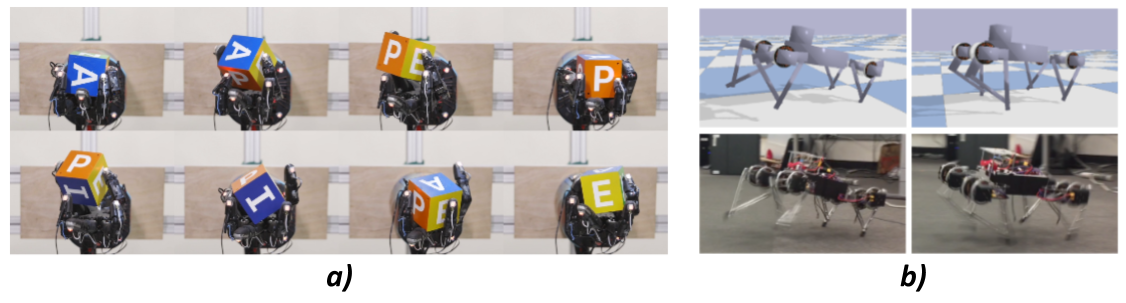
\includegraphics[width=6.0in,height=1.8in]{./chapters/imgs/img_reality_gap_approaches.png}
	\caption[Reality gap approaches]{Some approaches to solve for the reality gap. 
		a) Robotic hand generalizing in randomized environment \citep{dexterity-openai}.
		b) Quadruped trained in simulation and deployed in real world \citep{simtoreal-quadruped} }
	\label{fig:reality-gap-approaches}
\end{figure}

% @TAG: Refer to initial content and "emphazise" the objectives
\section{Objectives}
\label{sec:objectives}

\subsection*{General Objective}
Make a framework to build training and testing environments for continuous control tasks, and 
evaluate the performance and generalization capabilities of current state of the art DRL algorithms.

\subsection*{Specific Objectives}
\begin{itemize}
 \item Implement software tools on top of current RL APIs and physics engines 
       to create complex RL tasks for continuous control.
 \item Evaluate the performance of state of the art DRL algorithms in these environments.
\end{itemize}

\section{Organization}
\label{sec:organization}

The structure of this proposal is as follows :

\begin{itemize}
	\item @TODO: Overview chap2
	\item @TODO: Overview chap3
	\item @TODO: Overview chap4
	\item @TODO: Overview chap5
\end{itemize}